%%%%%%%% ICML 2024 STYLE PROGRESS REPORT %%%%%%%%%%%%%%%%%

\documentclass{article}
\usepackage[utf8]{inputenc}
\usepackage[english]{babel}
\usepackage{microtype}
\usepackage{graphicx}
\usepackage{booktabs}
\usepackage{array}
\usepackage{hyperref}
\usepackage{caption}
\usepackage{float}
\usepackage{xurl}
\Urlmuskip=0mu plus 2mu\relax
\newcommand{\code}[1]{\texttt{#1}}
\newcommand{\sourcerepo}{\href{https://github.com/bao-tg/COMP4040---Representation-Learning}{https://github.com/bao-tg/COMP4040---Representation-Learning}}
\makeatletter
\newcommand{\blfootnote}[1]{%
  \begingroup
  \renewcommand\thefootnote{}%
  \long\def\@makefntext##1{\noindent\raggedright ##1}%
  \footnotetext{#1}%
  \endgroup
}
\makeatother
\newcommand{\theHalgorithm}{\arabic{algorithm}}
\usepackage[accepted]{icml2024}
\usepackage{amsmath, amssymb, mathtools, amsthm}
\usepackage[capitalize,noabbrev]{cleveref}
\usepackage{tikz}
\usetikzlibrary{shapes.geometric, arrows.meta, positioning, shadows.blur}
\newcolumntype{P}[1]{>{\raggedright\arraybackslash}p{#1}}

\makeatletter
\setlength{\textfloatsep}{7pt plus 1pt minus 1pt}
\setlength{\floatsep}{7pt plus 1pt minus 1pt}
\setlength{\intextsep}{7pt plus 1pt minus 1pt}
\setlength{\dbltextfloatsep}{7pt plus 1pt minus 1pt}
\setlength{\dblfloatsep}{7pt plus 1pt minus 1pt}
\long\def\@makecaption#1#2{%
 \vskip 4pt
 \baselineskip 11pt
 \setbox\@tempboxa\hbox{#1. #2}
 \ifdim \wd\@tempboxa >\hsize
   \sbox{\newcaptionbox}{\small\sl #1.~}
   \newcaptionboxwid=\wd\newcaptionbox
   \usebox\newcaptionbox {\footnotesize #2}
 \else
   \centerline{{\small\sl #1.} {\small #2}}
 \fi}
\makeatother

\icmltitlerunning{Representation Learning on Amazon Reviews}

\begin{document}

\twocolumn[
\icmltitle{Representation Learning on Amazon Reviews 2023 \\
\textit{Natural Language / Clustering / Retrieval Analysis}}

\begin{icmlauthorlist}
\icmlauthor{Truong Gia Bao}{aaa}
\icmlauthor{Tran Quang Khai}{bbb}
\icmlauthor{Ngo Thanh An}{ccc}
\end{icmlauthorlist}

\icmlaffiliation{aaa}{21bao.tg@vinuni.edu.vn}
\icmlaffiliation{bbb}{23khai.tq@vinuni.edu.vn}
\icmlaffiliation{ccc}{24an.nt2@vinuni.edu.vn}

\icmlcorrespondingauthor{Truong Gia Bao}{21bao.tg@vinuni.edu.vn}
\icmlcorrespondingauthor{Tran Quang Khai}{23khai.tq@vinuni.edu.vn}
\icmlcorrespondingauthor{Ngo Thanh An}{24an.nt2@vinuni.edu.vn}

\icmlkeywords{Amazon Reviews, Representation Learning, Text Mining, Retrieval, Clustering}

\vskip 0.3in
]

\printAffiliationsAndNotice{}

\begin{abstract}
Text representation is a critical modeling choice in large-scale review mining, because each encoder imposes a different geometry on the same corpus. This project studies that choice on Amazon Reviews 2023~\cite{hou2024bridging}. We construct a reproducible pipeline over 2,000,000 raw reviews and obtain 1,946,618 cleaned review instances across five product categories. We compare five representative encoders from three major representation families: TF-IDF with TruncatedSVD as a sparse lexical baseline, Word2Vec and GloVe as static word-vector averaging methods, and SBERT and BGE-large as contextual sentence encoders. The frozen embeddings are evaluated under the same downstream pipeline: category-aligned clustering, semantic retrieval, UMAP visualization, runtime and storage efficiency, and a supervised linear probe for five-class star-rating prediction. Anomaly analysis is retained only as an auxiliary diagnostic.

The results show that no single representation dominates all tasks. SBERT achieves the strongest category-aligned clustering by NMI and ARI, while BGE-large gives the best semantic retrieval and star-rating linear-probe performance. TF-IDF remains useful for transparent category-specific lexical structure, and static word-vector averages provide lightweight semantic baselines but lose document-level composition. A corpus-trained Word2Vec/GloVe ablation further shows that target-domain training improves Word2Vec but degrades GloVe, suggesting that domain adaptation depends on the embedding objective and the available co-occurrence statistics. Overall, the project highlights a practical encoder-selection trade-off: BGE-large is best when retrieval quality or rating-relevant semantics justify high compute cost, SBERT is a strong quality--cost compromise, and TF-IDF remains a scalable lexical baseline.
\end{abstract}
\blfootnote{\textbf{GitHub repository:} \sourcerepo.}

\section{Introduction}

Representation learning is a central component of modern text mining systems because it determines how raw textual observations are converted into numerical forms that downstream algorithms can use. In text applications, this conversion is especially important: the quality of the representation affects whether documents with similar meanings are placed close together, whether latent category structure can be recovered, and whether unusual or inconsistent instances can be detected. Classical sparse representations such as TF-IDF remain widely used because they are simple, interpretable, efficient, and scalable \cite{salton1988}. However, they primarily capture lexical overlap and may fail to represent deeper semantic relationships between texts that use different surface forms.

Recent neural embedding models, including static word-vector methods and contextual sentence encoders, aim to address these limitations by mapping text into dense semantic vector spaces \cite{mikolov2013,pennington2014,vaswani2017,devlin2019}. Models such as Sentence-BERT and BGE-large are designed to capture sentence-level meaning and are therefore expected to perform better on semantic retrieval, clustering, and classification-style tasks \cite{reimers2019,xiao2023}. At the same time, these models require substantially greater computational resources, especially when applied to millions of documents. As a result, the practical value of a representation method depends not only on its predictive or semantic quality, but also on its runtime, memory footprint, and scalability.

This project empirically studies this trade-off using large-scale Amazon review data \cite{hou2024bridging}. Our central research question is: \textit{Do contextual embeddings reveal richer and more useful structure in large text corpora than sparse or static-vector representations, and what computational cost is required to obtain these gains?} To answer this question, we compare five encoding approaches: TF-IDF with dimensionality reduction, pretrained Word2Vec, pretrained GloVe, Sentence-BERT, and BGE-large. We evaluate these representations across clustering, semantic retrieval, UMAP visualization, efficiency analysis, and a supervised linear probe for five-class star-rating classification. The contribution of this project is not a new embedding model, but a controlled large-scale empirical comparison showing how representation choice changes conclusions across unsupervised structure discovery, retrieval, supervised probing, and computational cost.
\section{Dataset and Preprocessing}
\subsection{Dataset}
We use a sampled subset of Amazon Reviews 2023 \cite{hou2024bridging} containing five categories: Books, Electronics, Kindle Store, Movies and TV, and Sports and Outdoors. Each category contributes 400,000 raw rows, giving 2,000,000 raw reviews before cleaning. Reviews contain text, title, star rating, user/product identifiers, verified-purchase status, and category. Category is used as the external label for clustering and retrieval evaluation, while star rating is used for linear probing and auxiliary rating-inconsistency diagnostics. Raw category files were streamed from the public dataset to avoid loading the full compressed sources into memory. Because the sampling is intentionally category-balanced, the corpus should be interpreted as a controlled multi-category benchmark rather than as the natural Amazon review distribution.

\begin{table}[H]
\centering
\footnotesize
\setlength{\tabcolsep}{2pt}
\renewcommand{\arraystretch}{1.04}
\begin{tabular}{@{}P{0.32\linewidth}P{0.60\linewidth}@{}}
\toprule
Column & Role in this project \\
\midrule
text & Raw review body; cleaned text is the only encoder input \\
title & Metadata retained for inspection; not used as an encoder input \\
rating & Target for linear probe and auxiliary rating-inconsistency diagnostic \\
category & External label for clustering, retrieval, and UMAP coloring \\
user\_id & Used with product id and text for deduplication \\
asin, parent\_asin & Product identifiers; not used as model features \\
verified\_purchase & Metadata retained for inspection and validation \\
\bottomrule
\end{tabular}
\caption{Main dataset columns retained from Amazon Reviews 2023 and their use in the project.}
\label{tab:dataset-fields}
\end{table}

At the datapoint level, each instance is one product review. The encoder input is the cleaned review text, while the remaining fields are retained as metadata for evaluation, validation, or deduplication.

Encoders receive only the cleaned review text. Category and rating are retained as evaluation metadata: category is used for clustering, retrieval, and UMAP coloring, while rating is used for the linear probe and auxiliary rating-inconsistency diagnostic.

\subsection{Streaming preprocessing}
The preprocessing stage is implemented as a streaming pipeline so that the sampled JSONL files do not need to be loaded fully into memory. Each review is normalized by removing HTML-like tags, normalizing whitespace, trimming spaces, and truncating long reviews to at most 256 whitespace tokens. Rows with empty or very short cleaned text are removed using a minimum cleaned-text length of 10 characters. Cross-chunk deduplication is performed by hashing the tuple of user id, parent ASIN, and cleaned text. The final output is a single Parquet file containing 1,946,618 cleaned reviews and the metadata needed for downstream evaluation.

\begin{figure}[H]
\centering
\resizebox{\linewidth}{!}{%
    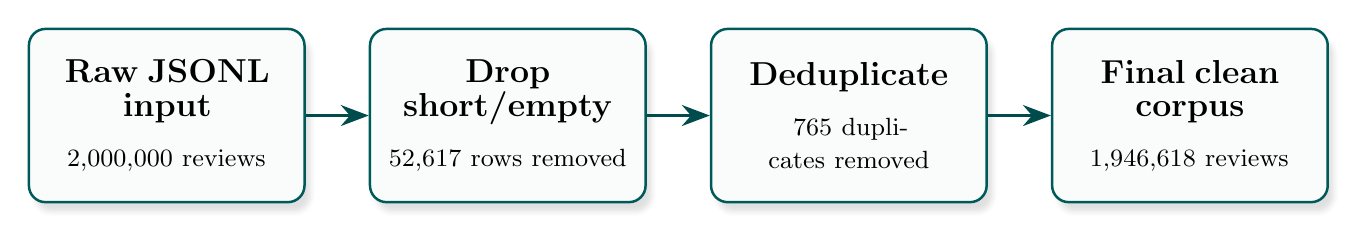
\begin{tikzpicture}[
        pipe/.style={
            rectangle,
            rounded corners=6pt,
            minimum width=3.5cm,
            minimum height=2.2cm,
            text width=3.2cm,
            align=center,
            draw=teal!70!black,         
            fill=teal!2!white,           
            line width=0.9pt,
            blur shadow={shadow opacity=12, shadow yshift=-0.8ex}
        },
        link/.style={
            -{Stealth[scale=1.2]},
            draw=teal!60!black,
            line width=1.2pt
        }
    ]
        \node (raw) [pipe] {\textbf{\large Raw JSONL input}\\[0.6em] {\small 2,000,000 reviews}};
        \node (drop) [pipe, right=0.8cm of raw] {\textbf{\large Drop short/empty}\\[0.6em] {\small 52,617 rows removed}};
        \node (dedup) [pipe, right=0.8cm of drop] {\textbf{\large Deduplicate}\\[0.6em] {\small 765 duplicates removed}};
        \node (final) [pipe, right=0.8cm of dedup] {\textbf{\large Final clean corpus}\\[0.6em] {\small 1,946,618 reviews}};

        \draw [link] (raw) -- (drop);
        \draw [link] (drop) -- (dedup);
        \draw [link] (dedup) -- (final);
    \end{tikzpicture}%
}
\caption{Streaming preprocessing flow and row counts. Short or empty reviews are removed before cross-chunk deduplication, producing the final cleaned corpus used by all downstream experiments.}
\label{fig:preprocess-flow}
\end{figure}

\vspace{-0.35em}
\begin{table}[H]
\centering
\footnotesize
\begin{tabular}{lcc}
\toprule
Category & Raw rows & Kept rows \\
\midrule
Books & 400,000 & 392,155 \\
Electronics & 400,000 & 390,822 \\
Kindle Store & 400,000 & 394,313 \\
Movies and TV & 400,000 & 378,924 \\
Sports and Outdoors & 400,000 & 390,404 \\
\midrule
Total & 2,000,000 & 1,946,618 \\
\bottomrule
\end{tabular*}
\caption{Full preprocessing output by category.}
\label{tab:preprocess}
\end{table}
\vspace{-0.35em}

Figure~\ref{fig:preprocess-flow} and Table~\ref{tab:preprocess} show that preprocessing is conservative rather than aggressive. The final corpus retains 97.33\% of the sampled rows, and the largest removal source is short or empty text rather than duplicate reviews. This matters because the downstream comparison is not driven by heavy filtering or by a major class imbalance introduced during cleaning. The kept category sizes remain close, ranging from 378,924 to 394,313 rows, so each encoder is evaluated on a broadly balanced five-category problem. At the same time, the category-specific drop rates are informative: Movies and TV loses 5.27\% of its rows, while Kindle Store loses only 1.42\%. This suggests that some categories contain more short, sparse, or noisy review text, which partly explains why category labels are useful but imperfect supervision signals for later clustering and retrieval analysis.

\section{Representation Methods and Formulation}
Let $d_i$ be a cleaned review and $z_i \in \mathbb{R}^p$ be its embedding. The project compares five encoders across three representation families.

The goal of this encoder selection is not to exhaustively benchmark every available text embedding model, but to compare representative points along the main design spectrum of text representation. TF-IDF tests whether large-scale review structure can already be recovered from lexical overlap and category-specific vocabulary. Word2Vec and GloVe test whether dense distributional word semantics improve over sparse lexical features when document vectors are built by simple averaging. SBERT tests a compact contextual sentence encoder optimized for semantic similarity, while BGE-large tests a larger retrieval-oriented contextual encoder with substantially higher capacity and cost. Therefore, the five encoders form a controlled progression from sparse lexical representations to static semantic averaging and finally to contextual sentence-level representations. This design allows us to ask not only which encoder performs best, but also which representation mechanism is useful for each data mining task.

\textbf{TF-IDF + TruncatedSVD.} The lexical baseline first builds a sparse TF-IDF matrix with the 10,000 most frequent non-stopword features \cite{salton1988}. The implementation follows the smoothed TF-IDF weighting used by scikit-learn \cite{pedregosa2011}:
\begin{equation}
\mathrm{tfidf}(t,d)=\mathrm{tf}(t,d)\left(1+\log \frac{1+N}{1+\mathrm{df}(t)}\right),
\end{equation}
where $N$ is the number of documents and $\mathrm{df}(t)$ is the number of documents containing term $t$. Rows are then normalized by the vectorizer. To make the representation comparable with dense methods, we compress the sparse matrix with TruncatedSVD, following latent semantic analysis and randomized SVD ideas \cite{deerwester1990,halko2011},
\begin{equation}
X \approx U_k \Sigma_k V_k^\top,
\end{equation}
using $k=300$ components. This method is fast and preserves category-specific vocabulary, but it does not explicitly model context or paraphrase.

\textbf{Pretrained static word vectors.} Word2Vec and GloVe provide 300-dimensional pretrained word vectors \cite{mikolov2013,pennington2014}. A review-level embedding is obtained by averaging available token vectors,
\begin{equation}
 z_d = \frac{1}{|T_d|}\sum_{w\in T_d} e_w,
\label{eq:mean-static}
\end{equation}
where $T_d$ is the whitespace-token sequence of review $d$ after out-of-vocabulary tokens are ignored, and $e_w$ is the pretrained vector of word $w$. Reviews with no covered tokens receive a zero vector. This captures broad lexical semantics but loses word order, syntax, negation, and word-sense context.

\textbf{Corpus-trained static-vector ablation.} To separate the effect of external pretraining from the static averaging architecture, we also train Word2Vec and GloVe variants on the cleaned Amazon review corpus for Table~\ref{tab:static-ablation}. These variants keep the same 300-dimensional document representation in Eq.~\eqref{eq:mean-static}: after token-level vectors are learned, each review is encoded by averaging the covered word vectors. Corpus Word2Vec is trained as a skip-gram model with window size 5, minimum token count 5, subsampling rate $10^{-3}$, random seed 42, and 5 epochs over the streamed cleaned corpus. Corpus GloVe first keeps the 50,000 most frequent tokens with minimum count 5, builds distance-weighted co-occurrence counts within a window of 5, and optimizes the weighted log-co-occurrence objective for 25 epochs using $x_{\max}=100$ and $\alpha=0.75$. Reviews with no covered trained-vocabulary tokens again receive a zero vector. This ablation therefore tests whether target-domain token vectors improve the same static document-composition method, rather than introducing a new document encoder.

\textbf{Contextual sentence embeddings.} Contextual sentence encoders build on Transformer and BERT-style representation learning \cite{vaswani2017,devlin2019}. SBERT all-MiniLM-L6-v2 outputs 384-dimensional sentence embeddings optimized for semantic similarity \cite{reimers2019,wang2020minilm}. BGE-large, \code{BAAI/bge-large-en-v1.5}, outputs 1024-dimensional embeddings and is designed for high-quality semantic retrieval \cite{xiao2023}. We encode the cleaned review text directly, without adding a retrieval prompt, so that the same representation can be reused across clustering, retrieval, visualization, linear probing, and auxiliary diagnostics. We expect BGE-large to perform strongly on retrieval and rating-related semantic tasks, but to be the most expensive encoder.

\section{Experimental Design}

\begin{figure*}[t]
\centering
\resizebox{\textwidth}{!}{%
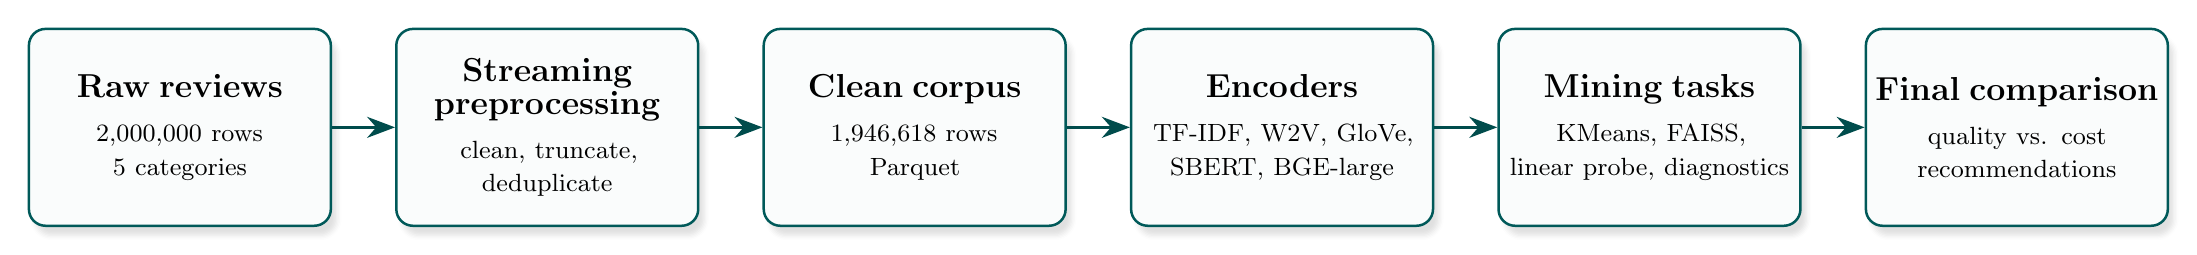
\begin{tikzpicture}[
    pipe/.style={
        rectangle,
        rounded corners=6pt,
        minimum width=3.8cm,
        minimum height=2.5cm,
        text width=3.6cm,
        align=center,
        draw=teal!70!black,         
        fill=teal!2!white,           
        line width=0.9pt,
        blur shadow={shadow opacity=12, shadow yshift=-0.8ex}
    },
    link/.style={
        -{Stealth[scale=1.2]},
        draw=teal!60!black,
        line width=1.2pt
    }
]

    \node (raw) [pipe] {
        \textbf{\large Raw reviews}\\[0.5em] 
        {\small 2,000,000 rows\\5 categories}
    };
    
    \node (stream) [pipe, right=0.8cm of raw] {
        \textbf{\large Streaming preprocessing}\\[0.5em] 
        {\small clean, truncate,\\deduplicate}
    };
    
    \node (clean) [pipe, right=0.8cm of stream] {
        \textbf{\large Clean corpus}\\[0.5em] 
        {\small 1,946,618 rows\\Parquet}
    };
    
    \node (encoder) [pipe, right=0.8cm of clean] {
        \textbf{\large Encoders}\\[0.5em] 
        {\small TF-IDF, W2V, GloVe,\\SBERT, BGE-large}
    };
    
    \node (tasks) [pipe, right=0.8cm of encoder] {
        \textbf{\large Mining tasks}\\[0.5em] 
        {\small KMeans, FAISS,\\linear probe, diagnostics}
    };
    
    \node (compare) [pipe, right=0.8cm of tasks] {
        \textbf{\large Final comparison}\\[0.5em] 
        {\small quality vs. cost\\recommendations}
    };

    \draw [link] (raw) -- (stream);
    \draw [link] (stream) -- (clean);
    \draw [link] (clean) -- (encoder);
    \draw [link] (encoder) -- (tasks);
    \draw [link] (tasks) -- (compare);

\end{tikzpicture}%
}
\caption{End-to-end experimental pipeline. The same cleaned Parquet corpus is encoded by all five representation methods, then reused for clustering, retrieval, visualization, linear probing, efficiency analysis, and auxiliary diagnostics.}
\label{fig:overall-pipeline}
\end{figure*}

Figure~\ref{fig:overall-pipeline} is important for interpreting the experiment because it keeps the comparison controlled. All encoders receive the same cleaned Parquet corpus, and each downstream task reuses the same frozen embedding arrays. Therefore, differences in Table~\ref{tab:main-results}, Figure~\ref{fig:umap-results}, and Table~\ref{tab:efficiency-results} can be attributed mainly to representation behavior rather than to different preprocessing paths. The pipeline also separates one-time encoding cost from reusable downstream analysis. This distinction is especially important for BGE-large: its quality gains are meaningful only if the expensive embedding stage can be reused for many retrieval, clustering, or prediction tasks.

\subsection{Clustering}
For each encoder, we fit MiniBatchKMeans with $K=5$ clusters, equal to the number of product categories \cite{macqueen1967,sculley2010}. The full run uses streaming mini-batches so that the entire embedding matrix does not need to be materialized in working memory beyond the memory-mapped array. The objective is
\begin{equation}
\min_{C_1,\ldots,C_K}\sum_{k=1}^K\sum_{x_i\in C_k}\|x_i-\mu_k\|_2^2.
\end{equation}
Cluster assignments are compared with product categories using normalized mutual information (NMI) and adjusted Rand index (ARI) \cite{strehl2002,hubert1985}. Silhouette score is computed on a 20,000-point sample for scalability \cite{rousseeuw1987}. UMAP is used for a 50,000-point stratified visualization sample \cite{mcinnes2018}.

\subsection{Semantic retrieval}
Semantic retrieval tests whether same-category reviews are close in embedding space. We build an exact FAISS L2 index over the full embedding matrix \cite{johnson2019}, sample 5,000 query reviews, and retrieve nearest neighbors from the full index. The query item itself is removed from the returned neighbor list when it appears as the nearest neighbor. A retrieval is relevant when it has the same category as the query. We do not normalize vectors for cosine similarity, so the reported numbers specifically evaluate L2 neighborhoods in each encoder's embedding space. We report
\begin{equation}
\mathrm{P@}k=\frac{1}{k}\sum_{j=1}^{k}\mathbf{1}[\ell_j=\ell_q],
\end{equation}
for $k \in \{5,10,50\}$, and mean reciprocal rank
\begin{equation}
\mathrm{MRR}=\frac{1}{|Q|}\sum_{q\in Q}\frac{1}{\mathrm{rank}_q},
\end{equation}
where $\ell_q$ is the query category, $\ell_j$ is the category of the $j$th retrieved item, and $\mathrm{rank}_q$ is the rank of the first relevant retrieved item.

\subsection{Auxiliary anomaly diagnostics}
We retain anomaly detection only as an auxiliary diagnostic. Isolation Forest is fit on a 200,000-row sample with fixed contamination $0.01$, and a scalable L2 SGDRegressor estimates rating residuals from frozen embeddings \cite{liu2008,bottou2010,pedregosa2011}. Because both views are threshold-driven and the corpus has already been cleaned for short text and duplicates, anomaly counts are not treated as encoder-quality metrics.

\subsection{Linear probe and efficiency}
The linear probe tests how much rating information is directly accessible from each frozen embedding. We train an L2-regularized logistic classifier,
\begin{equation}
\hat{y}=\arg\max_c \mathrm{softmax}(Wz_i+b)_c,
\end{equation}
with an 80/20 stratified train/test split and three epochs, implemented with stochastic-gradient linear models \cite{bottou2010,pedregosa2011}. In the full run this gives 1,557,294 training rows and 389,324 held-out test rows. Efficiency analysis records rows, dimensions, file size, device, and parsed embedding runtime.

\section{Results}

This section reports the full-scale results on 1,946,618 cleaned Amazon review rows. The primary comparison evaluates five encoders across category-aligned clustering, semantic retrieval, linear probing, UMAP visualization, and efficiency. Table~\ref{tab:main-results} summarizes the main quantitative findings. Overall, contextual encoders perform best, but the strongest encoder depends on the downstream task: SBERT is best for category-aligned clustering by NMI and ARI, while BGE-large is best for semantic retrieval and rating prediction. We also include a focused static-vector ablation comparing pretrained Word2Vec/GloVe with corpus-trained variants.

\begin{table*}[t]
\centering
\footnotesize
\begin{tabular*}{\textwidth}{@{\extracolsep{\fill}}lccccccccccc@{}}
\toprule
\multicolumn{3}{c}{Embedding} & \multicolumn{3}{c}{Clustering} & \multicolumn{4}{c}{Semantic Retrieval} & \multicolumn{2}{c}{Linear Probe} \\
\cmidrule(lr){1-3}\cmidrule(lr){4-6}\cmidrule(lr){7-10}\cmidrule(l){11-12}
Encoder & Dim & Size & NMI & ARI & Sil. & MRR & P@5 & P@10 & P@50 & Acc. & Macro-F1 \\
\midrule
TF-IDF + SVD & 300 & 2.18GB & 0.226 & 0.107 & 0.001 & 0.691 & 0.527 & 0.515 & 0.482 & 0.447 & 0.435 \\
Word2Vec & 300 & 2.18GB & 0.014 & 0.010 & 0.006 & 0.722 & 0.580 & 0.569 & 0.546 & 0.432 & 0.420 \\
GloVe & 300 & 2.18GB & 0.030 & 0.023 & \textbf{0.036} & 0.742 & 0.597 & 0.590 & 0.568 & 0.433 & 0.408 \\
SBERT & 384 & 2.78GB & \textbf{0.410} & \textbf{0.348} & 0.016 & 0.819 & 0.718 & 0.712 & 0.697 & 0.456 & 0.443 \\
BGE-large & 1024 & 7.43GB & 0.342 & 0.294 & 0.032 & \textbf{0.828} & \textbf{0.730} & \textbf{0.725} & \textbf{0.713} & \textbf{0.590} & \textbf{0.584} \\
\bottomrule
\end{tabular*} 
\caption{Full-scale summary on 1,946,618 cleaned reviews. The table reports the same non-redundant quality metric set used in the static-vector ablation: clustering metrics, retrieval metrics at multiple cutoffs, and linear-probe accuracy plus macro-F1. Retrieval uses 5,000 sampled query reviews against the full FAISS index.}
\label{tab:main-results}
\end{table*}

Table~\ref{tab:main-results} should not be read as a single leaderboard. It shows that the tasks reward different geometric properties of the embedding space. Clustering rewards global category separation, retrieval rewards local nearest-neighbor quality, and the linear probe rewards rating-relevant sentiment and evaluative information that is linearly accessible. Under this view, the results are coherent rather than contradictory: SBERT has the best global category alignment, BGE-large has the best local semantic neighborhoods and rating signal, TF-IDF keeps useful lexical category cues, and averaged static vectors provide some local semantic similarity but weak global organization.

\subsection{Clustering}

The clustering experiment evaluates whether unsupervised MiniBatchKMeans clusters align with the five product categories. SBERT achieves the strongest category-aligned clustering performance, with NMI 0.410 and ARI 0.348. This is 0.068 NMI and 0.054 ARI above BGE-large, which is the second strongest clustering encoder. TF-IDF is the best non-contextual baseline, with NMI 0.226 and ARI 0.107. In contrast, Word2Vec and GloVe perform weakly on category-alignment metrics, suggesting that simple averaging of static word vectors loses many category-specific cues needed for global cluster separation.

The result shows that category structure is not captured equally by all semantic representations. SBERT appears to form compact sentence-level regions that align well with product categories. BGE-large is also strong, but its main advantage appears more clearly in nearest-neighbor retrieval and rating prediction rather than in global KMeans separation. TF-IDF remains useful because product categories often contain distinctive lexical signals, such as product names and domain-specific vocabulary.

Silhouette scores are low for all encoders, so they should be interpreted carefully. GloVe has the highest silhouette value in Table~\ref{tab:main-results}, but its NMI and ARI are much lower than the contextual encoders, meaning its clusters are not well aligned with the external category labels. Amazon review categories naturally overlap: Books and Kindle Store share vocabulary, Movies and TV reviews can discuss books or devices, and Sports and Outdoors reviews can contain general lifestyle language. Therefore, NMI and ARI are more informative than silhouette for this category-alignment experiment.

\begin{figure*}[t]
\centering
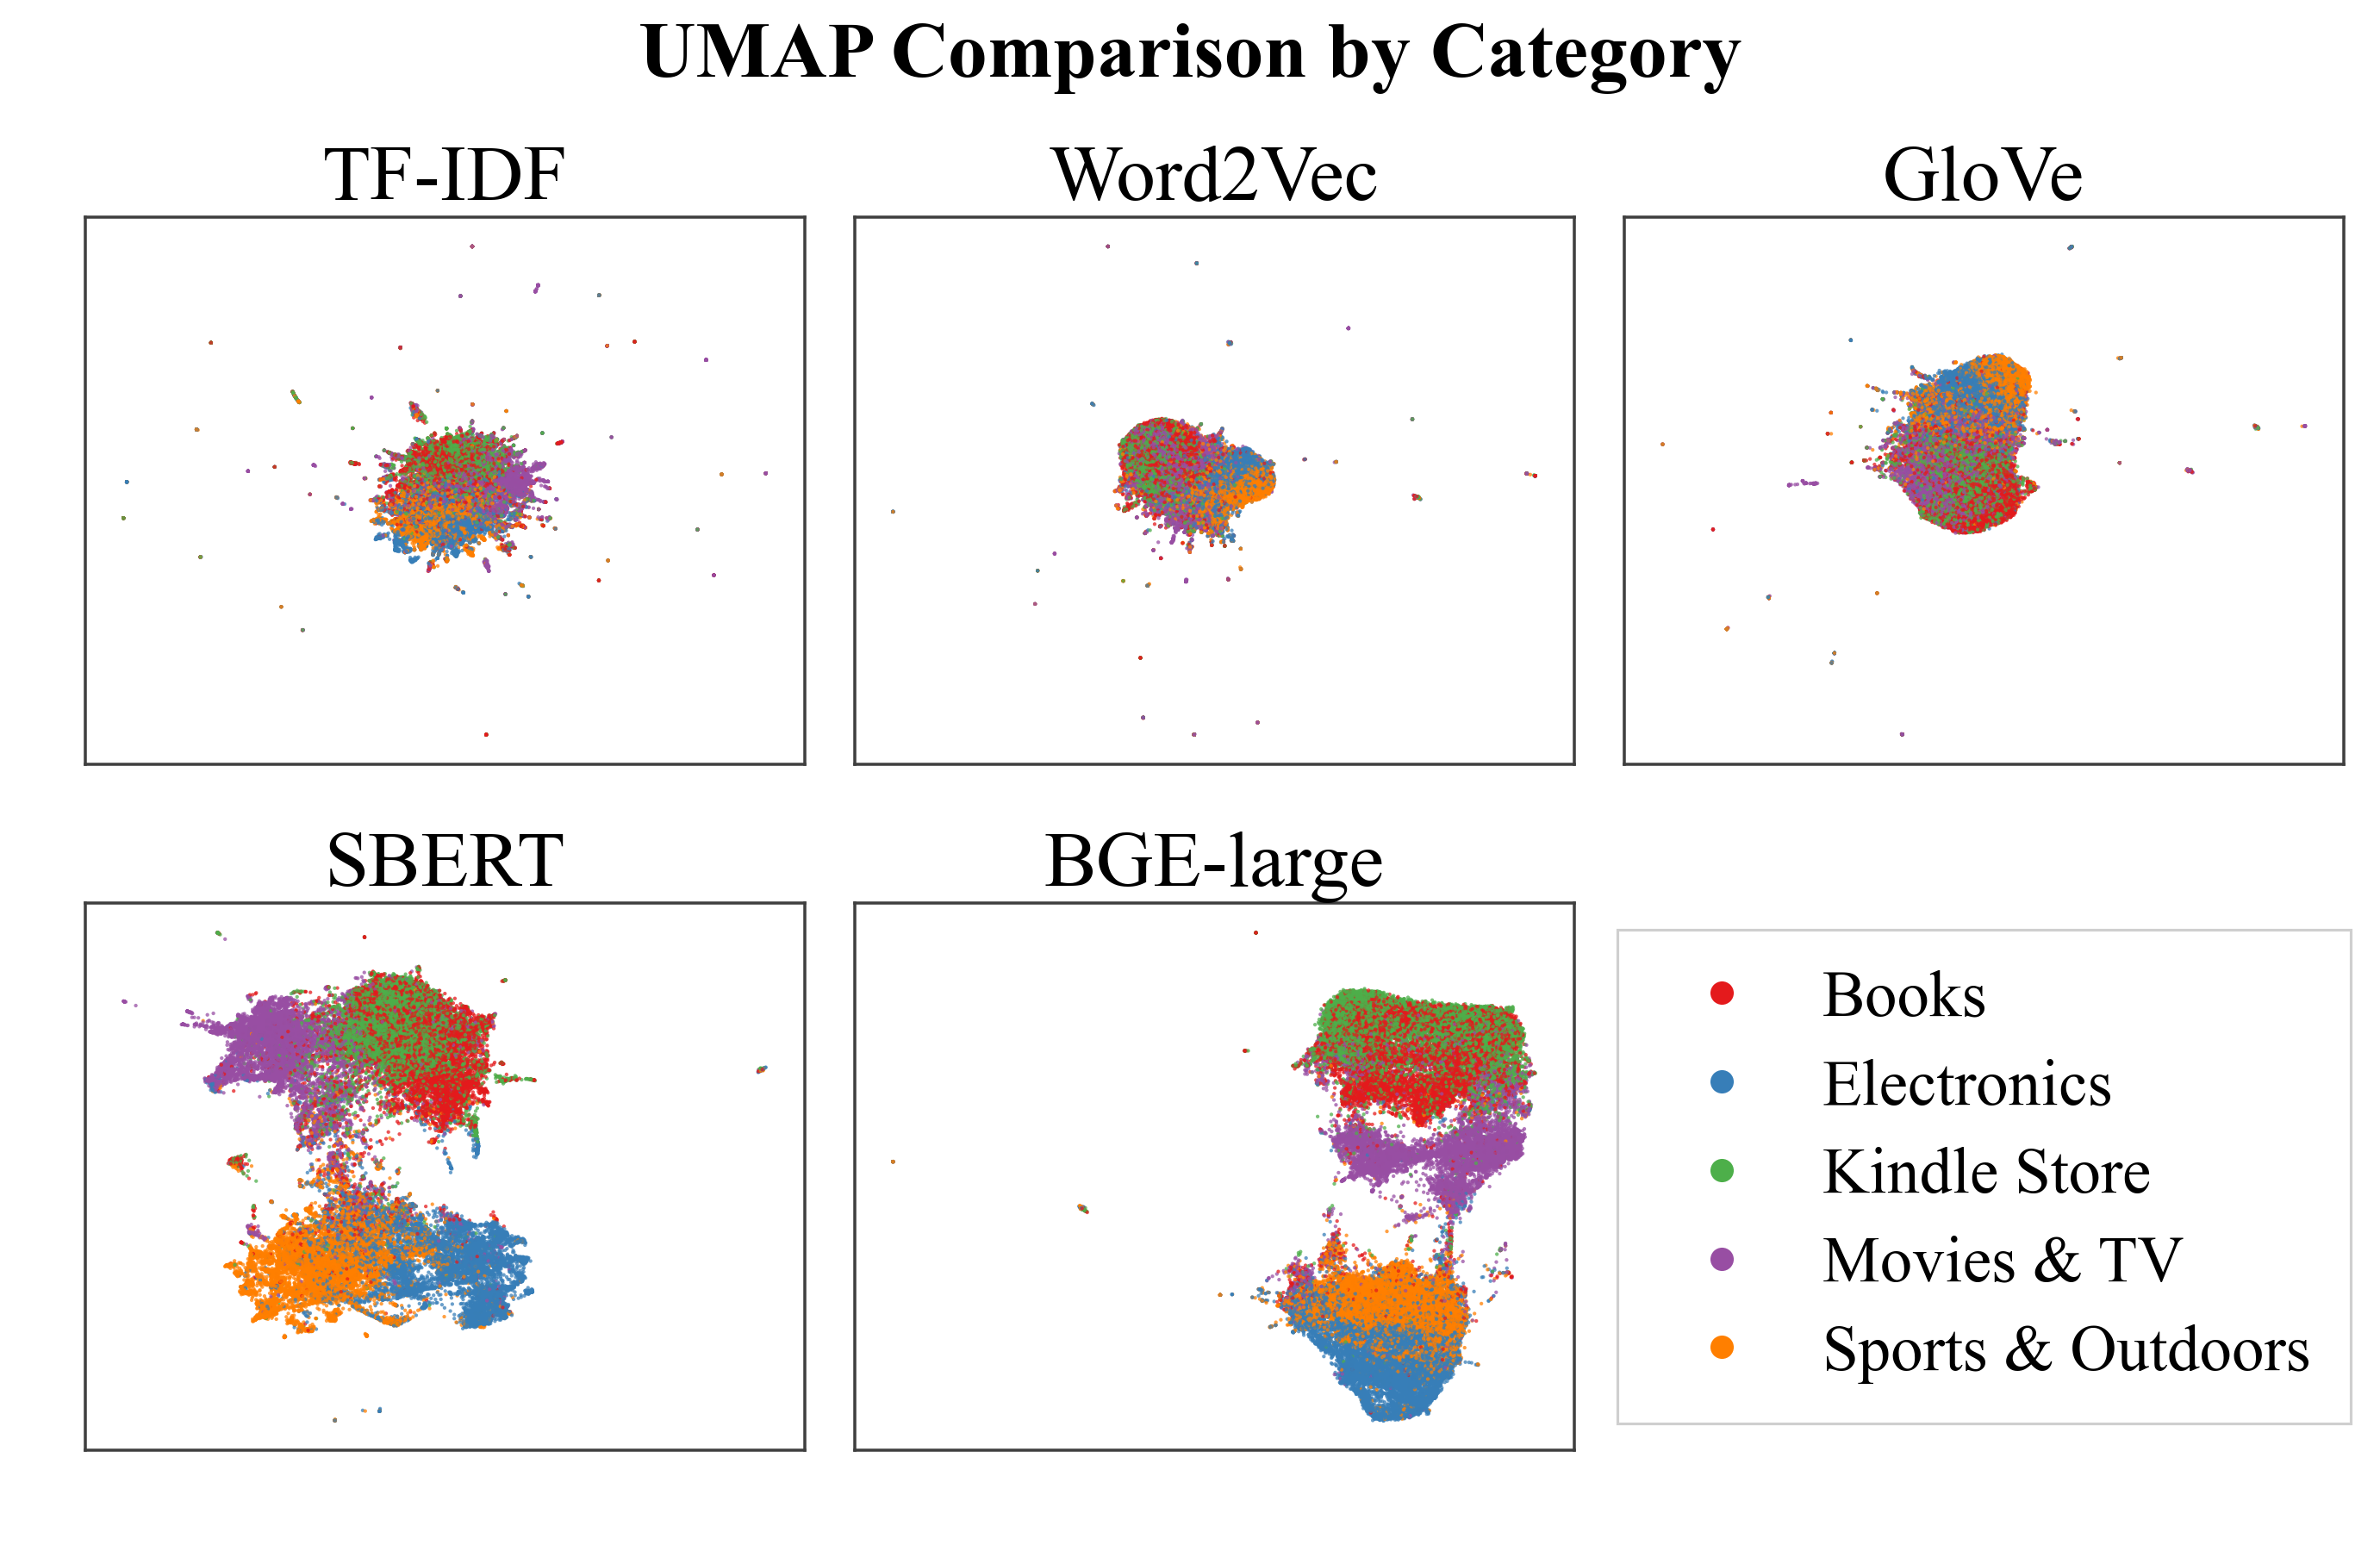
\includegraphics[width=0.49\textwidth]{figures/all_encoders_umap_category_grid.png}%
\hfill
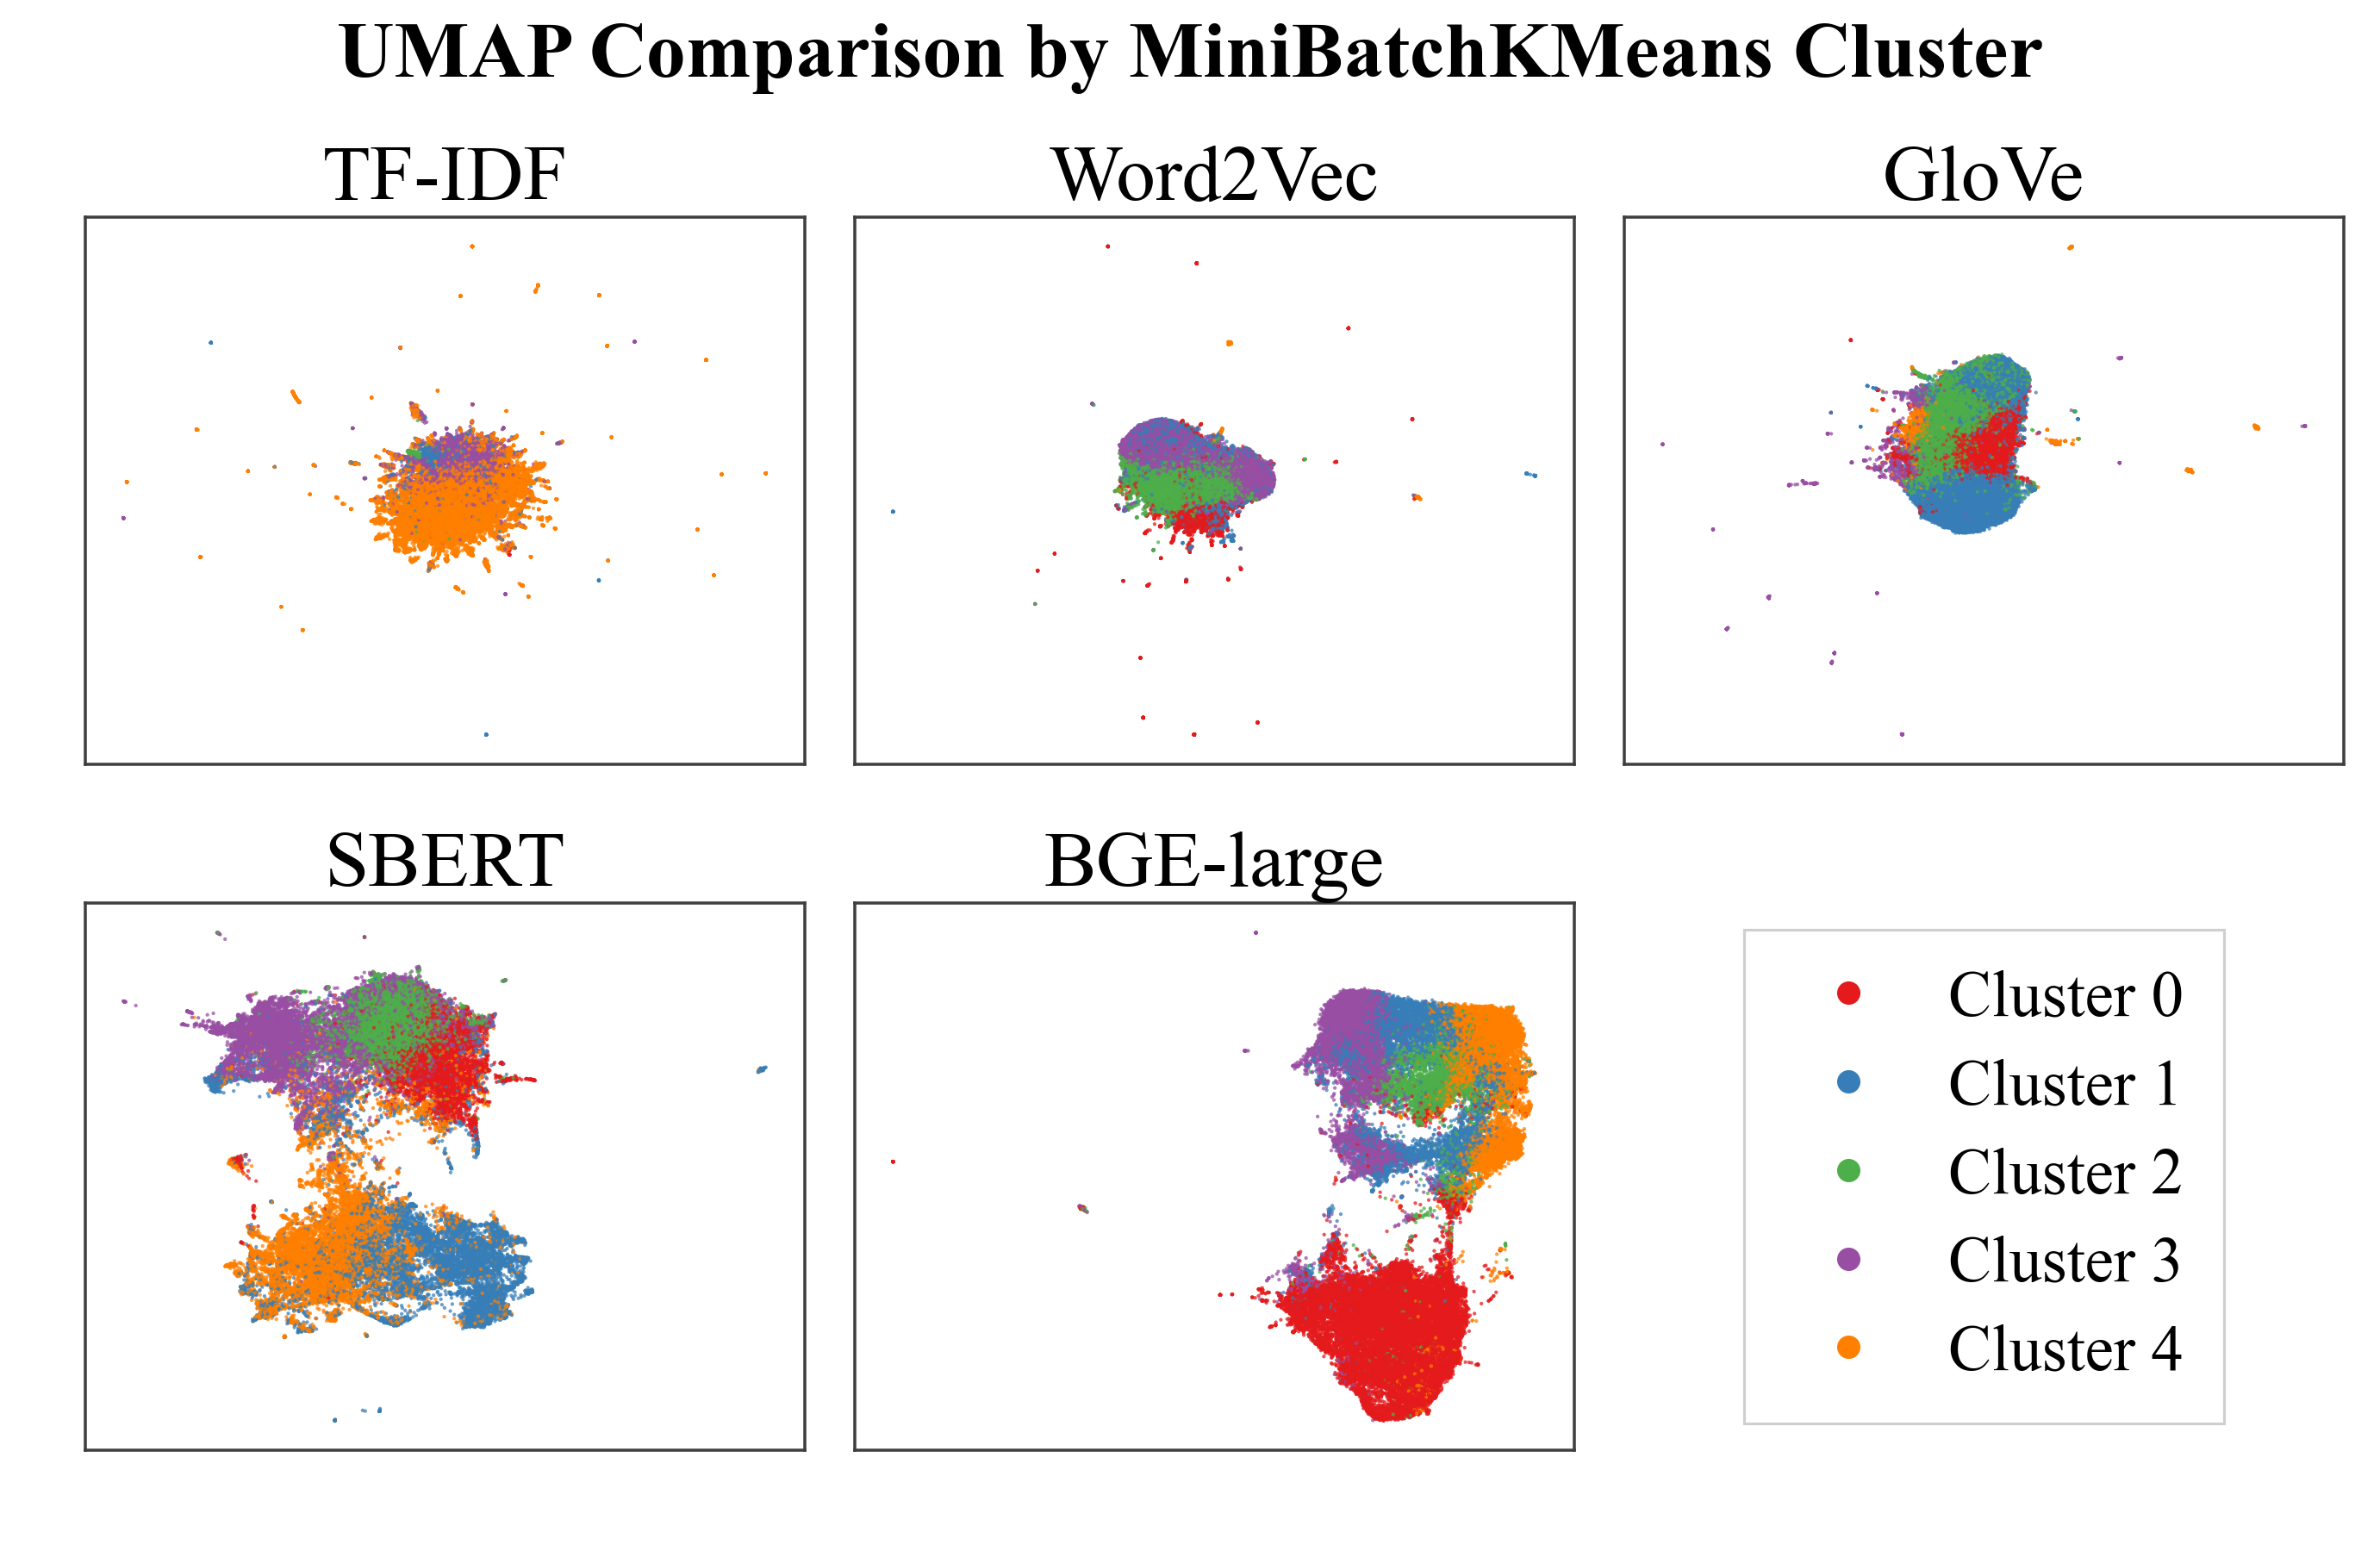
\includegraphics[width=0.49\textwidth]{figures/all_encoders_umap_cluster_grid.png}%
\caption{UMAP visualization on a 50,000-point stratified sample. Left: points colored by product category. Right: points colored by MiniBatchKMeans cluster assignment. These plots provide qualitative support for the clustering metrics.}
\label{fig:umap-results}
\end{figure*}

Figure~\ref{fig:umap-results} explains why the clustering metrics differ across encoders. In the category-colored panels, TF-IDF, Word2Vec, and GloVe show substantial mixing, which matches their weaker NMI and ARI values. TF-IDF still preserves some category-specific lexical structure, but the cloud remains compact and overlapping. Word2Vec and GloVe are even less category-aligned because averaging word vectors collapses many reviews with different document-level meanings into nearby regions. SBERT produces the clearest category-level organization, with larger separated regions, which is consistent with its best NMI and ARI. BGE-large also creates visible structure, but its geometry is more elongated and locally organized, which helps nearest-neighbor retrieval while being less ideal for a five-centroid KMeans partition. The cluster-colored panels reinforce this point: KMeans follows the geometry of each embedding space, not the ground-truth category labels. Thus, the UMAP figure is not only decorative; it visually shows the difference between local semantic structure and global category separability.

\subsection{Semantic Retrieval}

The retrieval experiment evaluates whether nearest neighbors in embedding space belong to the same product category as the query review. This task emphasizes local neighborhood quality rather than global cluster separation. BGE-large performs best across all retrieval metrics, with MRR 0.828, Precision@5 0.730, Precision@10 0.725, and Precision@50 0.713. SBERT is a close second, with MRR 0.819 and Precision@5 0.718. The gap between BGE-large and SBERT is small, only 0.009 MRR and 0.012 Precision@5, but BGE-large is consistently ahead. This suggests that BGE-large's retrieval-oriented training improves fine-grained local neighborhoods, even when category-level clustering is stronger for SBERT.

The retrieval ranking differs from the clustering ranking. Static pretrained embeddings, especially GloVe, outperform TF-IDF on retrieval even though they perform poorly on clustering. GloVe reaches MRR 0.742 and Precision@5 0.597, while Word2Vec reaches MRR 0.722 and Precision@5 0.580. This suggests that external pretrained word-vector knowledge helps local semantic similarity. However, because Word2Vec and GloVe use simple averaged document vectors, they still lose word order, syntax, negation, and context-dependent meaning. Contextual encoders remain clearly stronger for retrieval.

\subsection{Linear Probe}

The linear probe evaluates how much rating-relevant information is linearly accessible from each frozen embedding. This task gives the clearest advantage to BGE-large. BGE-large achieves accuracy 0.590 and macro-F1 0.584 on the held-out test set. The next strongest model is SBERT, with accuracy 0.456 and macro-F1 0.443. The improvement over SBERT is 0.134 accuracy and 0.141 macro-F1, which is much larger than BGE-large's retrieval margin over SBERT. TF-IDF is close to SBERT, reaching accuracy 0.447 and macro-F1 0.435, while Word2Vec and GloVe are slightly weaker.

This result is important because star rating is different from product category. Category-aligned clustering rewards broad domain separation, while rating prediction requires sentiment, evaluation, and fine-grained review semantics. The fact that BGE-large is much stronger on the linear probe suggests that it preserves more information about evaluative language, sentiment intensity, and review-level meaning. This also explains why the best encoder depends on the task: SBERT is best for category clustering, while BGE-large is best for retrieval and rating prediction.

\subsection{Corpus-Trained Static-Vector Ablation}

Table~\ref{tab:static-ablation} compares pretrained and corpus-trained Word2Vec/GloVe variants using the same 300-dimensional averaged word-vector document representation. Runtime is not used as a direct comparison because the corpus-trained variants were run locally after the original server experiment.

\begin{table*}[t]
\centering
\footnotesize
\begin{tabular*}{\textwidth}{@{\extracolsep{\fill}}llccccccccc@{}}
\toprule
\multicolumn{2}{c}{Static Encoder} & \multicolumn{3}{c}{Clustering} & \multicolumn{4}{c}{Semantic Retrieval} & \multicolumn{2}{c}{Linear Probe} \\
\cmidrule(lr){1-2}\cmidrule(lr){3-5}\cmidrule(lr){6-9}\cmidrule(l){10-11}
Encoder & Source & NMI & ARI & Sil. & MRR & P@5 & P@10 & P@50 & Acc. & Macro-F1 \\
\midrule
Word2Vec & Google News & 0.014 & 0.010 & 0.006 & 0.722 & 0.580 & 0.569 & 0.546 & 0.432 & 0.420 \\
Word2Vec & Amazon reviews & \textbf{0.143} & \textbf{0.119} & 0.032 & \textbf{0.752} & \textbf{0.613} & \textbf{0.602} & \textbf{0.579} & \textbf{0.492} & \textbf{0.481} \\
GloVe & Common Crawl 840B & 0.030 & 0.023 & \textbf{0.036} & 0.742 & 0.597 & 0.590 & 0.568 & 0.433 & 0.408 \\
GloVe & Amazon reviews & 0.007 & 0.004 & -0.014 & 0.618 & 0.430 & 0.415 & 0.373 & 0.308 & 0.286 \\
\bottomrule
\end{tabular*}
\caption{Static-vector ablation comparing external pretrained vectors with vectors trained on the Amazon review corpus. The table reports the same non-redundant quality metric set as Table~\ref{tab:main-results}. Local runtime for the corpus-trained variants is excluded from the hardware-controlled efficiency comparison.}
\label{tab:static-ablation}
\end{table*}

The ablation shows that target-domain training is not uniformly beneficial; its effect depends on the match between the learning objective and the available corpus. Corpus-trained Word2Vec improves every reported quality metric over pretrained Word2Vec: NMI rises from 0.014 to 0.143, ARI from 0.010 to 0.119, MRR from 0.722 to 0.752, and macro-F1 from 0.420 to 0.481. This improvement is not caused by dimensionality or by a different document encoder, since both versions remain 300-dimensional averaged word-vector representations. Instead, the likely gain comes from local domain adaptation: skip-gram Word2Vec repeatedly predicts nearby review tokens, so it can learn product names, category-specific phrases, rating adjectives, and Amazon-style evaluative language that are missing or differently weighted in Google News pretraining. Because document vectors are simple averages, better in-domain token coverage and better local token neighborhoods directly improve the review-level representation.

Corpus-trained GloVe shows the opposite pattern. It underperforms pretrained GloVe on all reported metrics, with particularly large drops in retrieval and rating prediction, and its silhouette score becomes negative. This does not mean that GloVe is inherently weak; rather, it shows that GloVe's global co-occurrence objective is more demanding under our data regime. Pretrained GloVe benefits from the broad Common Crawl 840B co-occurrence matrix, while our trained variant must estimate global co-occurrence statistics from a much narrower, review-only corpus with a practical 50,000-token vocabulary cap. As a result, the model can overemphasize frequent review boilerplate and product-domain co-occurrences while losing broad semantic relations and long-tail lexical coverage. The deeper conclusion is therefore about objective--data fit: Word2Vec's local predictive objective transfers well to a medium-scale domain corpus, whereas GloVe's matrix-factorization objective needs broader and more stable co-occurrence evidence to outperform a large external pretrained model.

\subsection{Efficiency and Scalability}

The efficiency results show the cost side of the representation-quality tradeoff. In Table~\ref{tab:efficiency-results}, encoding runtime is the wall-clock time needed to produce the frozen embedding matrix, excluding downstream clustering, retrieval, UMAP, linear probing, and report generation. Transformer encoders use pretrained weights but still tokenize and run a forward pass over every review; static baselines only vectorize text or average word vectors. Storage scales with dimension: the 300-dimensional baselines occupy 2.18GB, SBERT occupies 2.78GB, and BGE-large occupies 7.43GB.

\begin{table}[H]
\centering
\footnotesize
\setlength{\tabcolsep}{3pt}
\renewcommand{\arraystretch}{1.02}
\begin{tabular*}{\columnwidth}{@{\extracolsep{\fill}}lcccc@{}}
\toprule
Encoder & Device & Dim & Size (GB) & Runtime \\
\midrule
TF-IDF & CPU & 300 & 2.18 & 00:05:09 \\
Word2Vec & CPU & 300 & 2.18 & 00:02:31 \\
GloVe & CPU & 300 & 2.18 & 00:01:57 \\
SBERT & CUDA & 384 & 2.78 & 03:01:27 \\
BGE-large & CUDA & 1024 & 7.43 & 65:56:44 \\
\bottomrule
\end{tabular*}
\caption{Embedding efficiency summary from the full run. Runtime measures only embedding construction. Transformer encoders load pretrained weights but still compute embeddings for every review; static baselines only vectorize text or average pretrained word vectors.}
\label{tab:efficiency-results}
\end{table}

BGE-large gives the best retrieval and linear-probe performance, but this quality comes with a substantial computational cost. Its embedding stage required about 66 hours on CUDA in this run, roughly 21.8 times longer than SBERT, because the larger Transformer had to encode nearly two million review texts. This is an important tradeoff because BGE-large's retrieval gains over SBERT are modest, while its rating-prediction gains are large. Therefore, BGE-large is easiest to justify when rating-relevant semantics or the best possible retrieval quality are central to the application and the embeddings will be reused many times. SBERT is much cheaper while still achieving the best category-aligned clustering performance and strong retrieval performance. TF-IDF remains useful as a transparent and efficient lexical baseline, especially when the task benefits from category-specific vocabulary and interpretability.

Overall, the results support the main hypothesis that contextual embeddings discover richer structure than sparse or static representations. However, they also show that the definition of a better representation depends on the data mining task. SBERT best captures category-level cluster structure, BGE-large best supports nearest-neighbor retrieval and star-rating prediction, and TF-IDF remains competitive when category-specific vocabulary is important.

\section{Discussion}
The main finding is that no single representation dominates. SBERT is strongest for category clustering, BGE-large for retrieval and rating prediction, TF-IDF for category-specific lexical signals, and static word-vector averages are lightweight but less reliable.

The SBERT--BGE-large contrast is important. BGE-large has the strongest nearest-neighbor and rating-prediction performance, consistent with its retrieval-oriented training. However, SBERT produces more category-aligned clusters. One possible explanation is that SBERT's compact sentence embeddings smooth reviews into category-level semantic regions, while BGE-large preserves more fine-grained local similarity that is excellent for retrieval but less ideal for global KMeans separation. This means downstream task choice should guide encoder selection.

The static baselines show another tradeoff. Pretrained Word2Vec and GloVe perform reasonably well in retrieval because they bring external semantic knowledge. However, simple averaging ignores word order, syntax, negation, and sentence-level composition. TF-IDF behaves differently: it is weaker than contextual encoders for retrieval but stronger than static averages for clustering, because categories often contain distinctive keywords.

Embedding dimension should not be interpreted as the only explanation for performance. The experiment uses the standard off-the-shelf dimensionality of each encoder: 300 for TF-IDF/SVD, Word2Vec, and GloVe, 384 for SBERT, and 1024 for BGE-large. This makes the comparison realistic for deployment, but it is not a dimension-matched ablation. The results do not show a simple dimension--performance correlation: BGE-large has the largest dimension and is best for retrieval and linear probing, but SBERT has only 384 dimensions and is best for category-aligned clustering. Among the 300-dimensional methods, TF-IDF is stronger for clustering, while GloVe is stronger for retrieval. Therefore, architecture, pretraining objective, and document-composition method matter at least as much as dimensionality, although higher dimension clearly increases storage and runtime cost.

\section{Scalability and Complexity}
At full scale, the pipeline must be streaming and reusable. Preprocessing runs in chunks and writes Parquet, avoiding memory pressure from the two-million-row raw corpus. Embeddings are saved as \code{.npy} arrays with metadata so downstream experiments can be repeated without re-encoding. This design is important because BGE-large alone required about 66 hours to encode.

Theoretical complexity explains the observed cost pattern. TF-IDF is mostly linear in the number of tokens plus the cost of truncated SVD over a sparse term-document matrix. Static embedding averages are linear in the number of tokens times embedding dimension after vectors are loaded. Transformer encoders are more expensive because self-attention scales approximately quadratically with sequence length within each forward pass \cite{vaswani2017}. Downstream methods also scale with data size: exact FAISS L2 retrieval indexes all embeddings \cite{johnson2019}, MiniBatchKMeans scales with rows, clusters, dimensions, and passes \cite{sculley2010}, and auxiliary Isolation Forest diagnostics are made practical by fitting on a sample before scoring the full matrix \cite{liu2008}.

\section{Limitations}
First, category labels are used as retrieval relevance labels, but same-category reviews are not always semantically similar and different-category reviews can discuss similar concepts. Second, star ratings are noisy sentiment labels; a three-star review can contain mixed positive and negative evidence. Third, the raw sample is category-balanced by design, so it is useful for controlled comparison but does not preserve the natural Amazon category or product distribution. Fourth, Word2Vec and GloVe are represented by simple averaged word vectors, so stronger document-level static baselines might narrow the gap. Fifth, embedding dimensions are not matched across encoders; this is a practical off-the-shelf comparison rather than a controlled equal-dimensional ablation. Sixth, retrieval is evaluated with exact L2 neighborhoods only; cosine-normalized retrieval and BGE prompt variants may change the retrieval ranking. Seventh, we did not run exhaustive hyperparameter searches or repeated-seed confidence intervals for KMeans, UMAP, or the linear probe. Eighth, the corpus-trained static-vector ablation trains word vectors on the full cleaned corpus without category or rating labels; therefore, the linear-probe results should be interpreted as an unsupervised representation-learning setting rather than a strictly train-split-only supervised setting. Ninth, the corpus-trained Word2Vec and GloVe ablation was run locally after the original server experiment, so its runtime is reported only as a reproducibility reference and not as a hardware-controlled efficiency comparison. Finally, the anomaly outputs are retained only as qualitative diagnostics because fixed thresholds largely control the number of flagged rows.

\section{Conclusion}
This project scales the representation-learning pipeline from a small prototype to a full run over 1,946,618 cleaned Amazon reviews. The results support the original hypothesis that contextual embeddings reveal richer structure than sparse or static representations, but they also show that encoder choice is task-dependent: SBERT is strongest for category-aligned clustering, BGE-large is strongest for retrieval and rating prediction, and TF-IDF remains a transparent lexical baseline. The corpus-trained static-vector ablation further shows that target-domain training can help Word2Vec but does not automatically improve all static-vector methods, since corpus-trained GloVe underperforms its broad pretrained counterpart. Overall, encoder choice should be treated as a modeling decision rather than a default preprocessing step because each representation imposes different geometric assumptions on the same corpus.


\section*{Contributions}

All members contributed to project planning, debugging, result interpretation, and final writing. Each member owned one or more encoder families and ran the full experimental suite for the assigned encoder(s) on the two-million-row corpus.

\begin{itemize}
    \item \textbf{Truong Gia Bao:} Set up the project outline, formulated the research problem, designed the overall evaluation plan, and implemented and ran the TF-IDF representation baseline through the full-scale experiments.
    \item \textbf{Ngo Thanh An:} Implemented and ran the pretrained and corpus-trained Word2Vec and GloVe representation baselines through the full-scale experiments, including embedding generation, static-vector ablation, and downstream evaluation.
    \item \textbf{Tran Quang Khai:} Implemented and ran the SBERT and BGE-large contextual representation baselines through the full-scale experiments, including GPU embedding generation and downstream evaluation.
\end{itemize}

\newpage

\begingroup
\sloppy
\emergencystretch=3em
\bibliographystyle{icml2024}
\bibliography{references}
\endgroup

\end{document}
